\thispagestyle{empty}

\noindent
\begin{tabular}{@{}p{11cm}r@{}}
\textbf{ಡಾ. ಎಂ.ಜಿ. ಮಂಜುನಾಥ್,}\newline ಪ್ರಾಧ್ಯಾಪಕರು, ಕುವೆಂಪು ಕನ್ನಡ ಅಧ್ಯಯನ ಸಂಸ್ಥೆ,\newline ನಿರ್ದೇಶಕರು, ಪ್ರಸಾರಾಂಗ,\newline ಮೈಸೂರು ವಿಶ್ವವಿದ್ಯಾನಿಲಯ, ಮೈಸೂರು. & \raisebox{-2cm}{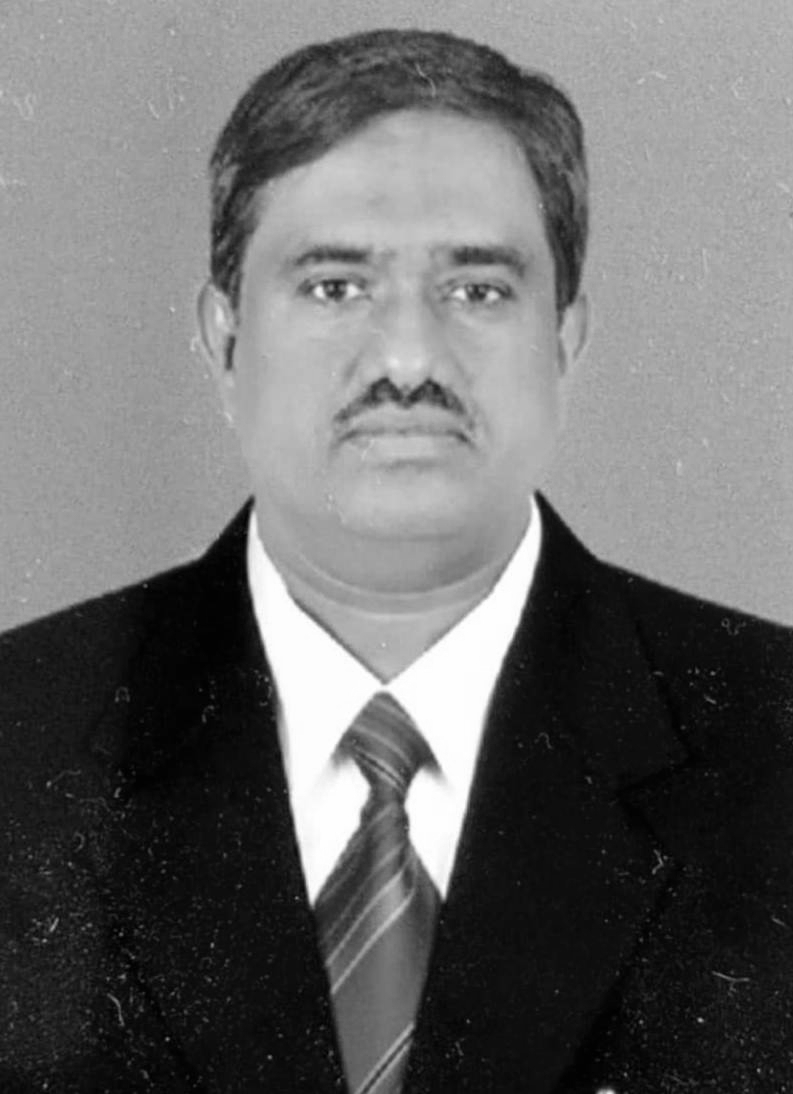
\includegraphics{"images/manjunath.jpg"}}
\end{tabular}

\noindent
\rule{\textwidth}{1pt}

\bigskip

ಮಂಡ್ಯ ಜಿಲ್ಲೆ, ಕೃಷ್ಣರಾಜಪೇಟೆ ತಾಲ್ಲೂಕು, ಸಂತೇಬಾಚಹಳ್ಳಿ ಗ್ರಾಮದಲ್ಲಿ ಜನಿಸಿದ ಅಪ್ಪಟ ಗ್ರಾಮೀಣ ಪ್ರತಿಭೆಯಾದ ಶ್ರಿ ಎಸ್​. ನಂಜುಂಡಸ್ವಾಮಿಯವರು ಶ್ರಮ ಸಂಸ್ಕೃತಿಯ ಆರಾಧಕ.   ತಮ್ಮ ಹಲವು ವರ್ಷಗಳ ಪರಿಶ್ರಮದ ಫಲಿತವಾಗಿ “ಮಂಡ್ಯ ಜಿಲ್ಲೆಯ ಶಾಸನಗಳು-ಒಂದು ಅಧ್ಯಯನ” ಎಂಬ ಮಹಾಪ್ರಬಂಧವನ್ನು ರಚಿಸಿ ಪಿಎಚ್​.ಡಿ. ಪದವಿಯನ್ನು ಪಡೆದು ಡಾ. ಎಸ್​. ನಂಜುಂಡಸ್ವಾಮಿಯಾಗಿದ್ದಾರೆ. ವೃತ್ತಿಯಿಂದ ಕರ್ನಾಟಕ ವಿಧಾನ ಮಂಡಲದ, ವಿಧಾನ ಪರಿಷತ್ತಿನಲ್ಲಿ ಅಧಿಕಾರಿಯಾಗಿದ್ದ ನಂಜುಂಡಸ್ವಾಮಿಯವರು, ಪ್ರವೃತ್ತಿಯಿಂದ ಒಬ್ಬ ನಿಷ್ಠಾವಂತ ಸಂಶೋಧಕ. ಸತತಾಭ್ಯಾಸ, ವ್ಯುತ್ಪತ್ತಿ, ಪರಿಶ್ರಮ ಮತ್ತು  ವ್ಯಾಪಕ ಕ್ಷೇತ್ರಕಾರ್ಯದ ಫಲಿತವಾಗಿ ಈ ಮಹಾಪ್ರಬಂಧವನ್ನು ರಚಿಸಿದ್ದಾರೆ. ಮಂಡ್ಯ ಜಿಲ್ಲೆಯಲ್ಲಿ ದೊರೆತಿರುವ ಎಲ್ಲ ಶಾಸನಗಳನ್ನೂ ತಲಸ್ಪರ್ಷಿಯಾಗಿ ಅಧ್ಯಯನ ಮಾಡಿರುವ ನಂಜುಂಡಸ್ವಾಮಿಯವರು, ಆ ಶಾಸನಗಳು ಇರುವ ಸ್ಥಳಗಳ\-ಲ್ಲೆಲ್ಲಾ ಕ್ಷೇತ್ರ ಪರಿವೀಕ್ಷಣೆ ಮಾಡಿದ್ದಾರೆ. ಸಾವಿರಾರು ಛಾಯಾಚಿತ್ರಗಳನ್ನು ತೆಗೆದಿದ್ದಾರೆ. ಅವುಗಳನ್ನೆಲ್ಲಾ ತಮ್ಮ ಮಹಾಪ್ರಬಂಧ ರಚನೆಗೆ ಬಳಸಿಕೊಂಡಿದ್ದಾರೆ.  ಈ ಸಂಶೋಧನೆಯು ಬಹುಶಿಸ್ತೀಯ ಮಾದರಿ ಸಂಶೋಧನೆಗೆ ಒಂದು ಅತ್ಯುತ್ತಮ ಉದಾಹರಣೆ ಎಂದು ಹೇಳಬಹುದು. ಪುರಾತತ್ತ್ವ ಶಾಸ್ತ್ರ, ಇತಿಹಾಸ, ಶಾಸನ ಶಾಸ್ತ್ರ, ವಾಸ್ತುಶಿಲ್ಪ ಶಾಸ್ತ್ರ, ಶಿಲ್ಪ ಶಾಸ್ತ್ರ, ಸಮಾಜ ಶಾಸ್ತ್ರ,  ಧಾರ್ಮಿಕ ಅಧ್ಯಯನ, ನೀರಾವರಿ ವ್ಯವಸ್ಥೆ, ಆರ್ಥಿಕ ಅಧ್ಯಯನ, ಸಾಹಿತ್ಯ ಅಧ್ಯಯನ ಹೀಗೆ ಹಲವು ಜ್ಞಾನಶಿಸ್ತುಗಳಿಗೆ ಸಂಬಂಧಿಸಿದಂತೆ ಈ ಮಹಾಪ್ರಬಂಧದಲ್ಲಿ ಸಮಗ್ರವಾಗಿ ವಿಶ್ಲೇಷಿಸಲಾಗಿದೆ. ಈ ಮಹಾಪ್ರಬಂಧದಲ್ಲಿನ ಪ್ರತಿಯೊಂದು ಅಧ್ಯಾಯವೂ ಒಂದೊಂದು\break ಪಿಎಚ್​.ಡಿ. ಸಂಶೋಧನೆಗೆ ಮಾರ್ಗದರ್ಶಕವಾಗಬಹುದಾದ ಅಧ್ಯಾಯಗಳಾಗಿವೆ. ನೂರಾರು ಬಿಡಿ ಸಂಶೋಧನಾ ಲೇಖನಗಳನ್ನು ರಚಿಸಲು ಆಕರ ಸಾಮಗ್ರಿಯನ್ನು ಒದಗಿಸುವಂತಹದಾಗಿವೆ. ತಮ್ಮ ಸಂಶೋಧನಾ ಪ್ರಬಂಧಕ್ಕೆ ಪಿಎಚ್​.ಡಿ. ಪಡೆದ ನಂತರವೂ ಸಹ ಈ ಕ್ಷೇತ್ರದಲ್ಲಿ ಮುಂದುವರಿಸಿದ ಸಂಶೋಧನೆ, ಅಧ್ಯಯನ, ಕ್ಷೇತ್ರಕಾರ್ಯಗಳ ಹಿನ್ನೆಲೆಯಲ್ಲಿ, ತಮ್ಮ ಮಹಾ ಪ್ರಬಂಧವನ್ನು ಪರಿಷ್ಕರಿಸಿ, ಅದರ ಫಲಿತವಾಗಿ \textbf{“ಮಂಡ್ಯ ಜಿಲ್ಲೆಯ ಶಾಸನ ಮತ್ತು ಸಂಸ್ಕೃತಿ”} ಎಂಬ ಮಹತ್ವದ ಸಂಶೋಧನಾ ಗ್ರಂಥ\-ವೊಂದನ್ನು ಕನ್ನಡ ಸಾರಸ್ವತ ಲೋಕಕ್ಕೆ ಕೊಡುಗೆಯಾಗಿ ನೀಡಿರುವ ಡಾ. ಎಸ್​. ನಂಜುಂಡಸ್ವಾಮಿಯವರಿಗೆ ಅಭಿನಂದನೆಗಳು.


\medskip
\bigskip

\noindent
\hfill \textbf{ಡಾ. ಎಂ.ಜಿ. ಮಂಜುನಾಥ್}

